\documentclass[a4paper, 12pt]{article}

\usepackage[utf8]{inputenc}
\usepackage[brazilian]{babel}
\usepackage{graphicx}
\usepackage{hyperref}
\usepackage[margin=2cm]{geometry}

% The following packages can be found on http:\\www.ctan.org
\usepackage{graphics} % for pdf, bitmapped graphics files
\usepackage{epsfig} % for postscript graphics files
\usepackage{mathptmx} % assumes new font selection scheme installed
\usepackage{times} % assumes new font selection scheme installed
\usepackage{amsmath} % assumes amsmath package installed
\usepackage{amssymb}  % assumes amsmath package installed
\usepackage[sort,comma]{natbib}
\usepackage{imakeidx}

\usepackage{xcolor}
\definecolor{myGreen}{RGB}{0,100,0}
\definecolor{myRed}{RGB}{230,0,0}
\definecolor{red}{RGB}{230,0,0}
\definecolor{blue}{RGB}{0,0,205}
\definecolor{myRed2}{RGB}{210,0,0}
\definecolor{myBlue}{RGB}{0,0,205}
\usepackage{setspace}
\usepackage{bm}
\usepackage{graphicx}
\bibliographystyle{plain}
\setlength{\parindent}{0.5cm}
\usepackage{proof}
\usepackage{alltt}


\pagestyle{plain}
\pagenumbering{arabic}
\makeindex

\title{\Huge \bf
Formalização e Propriedades do Algoritmo \textit{Radix Sort}
}

\author{\\\\
        \bf Universidade de Brasília\\
        \bf Departamento de Ciência da Computação\\
        \bf Lógica Computacional 1, Turma A\\
        \\\\
        Diogo Ferreira, 11/0027931\\
        Eduardo Freire, 16/0027136\\
        Gabriel Rocha, 15/0126760\\
        Juliana Hosoume, 18/0048864\\
        \\\\}
\date{\today}


\begin{document}
\maketitle
\thispagestyle{empty}

\begin{abstract}

O objetivo deste trabalho é relatar um meio de utilização do princípio de indução em Ciência da Computação para demonstrar formalmente a correção de \textit{merge sort} como algoritmo auxiliar estável para \textit{radix sort}. Para isso, foram aplicadas técnicas dedutivas da lógica de predicados, implementadas no assistente de demonstração PVS.

\end{abstract}

\newpage
\tableofcontents
\newpage

\section{Introdução e Contextualização do Problema}
\label{sec:Introducao}

O \textit{Radix Sort} é um algoritmo de ordenação rápido que processa as partes correspondentes de uma lista de itens com tipo predefinido. Em uma lista de inteiros, por exemplo, uma parte pode representar a significância dos dígitos de uma mesma posição, comparando-os e os ordenando em seguida. Neste caso, para ordená-los de modo crescente em relação ao valor de cada inteiro, usamos o método do dígito menos significativo - ordenamos primeiro as unidades, em seguida as dezenas, depois as centenas e assim por diante. Entretanto, este algorítimo necessita de um algoritmo auxiliar estável para ordenação das partes identificadas.

\begin{figure}[!h]
\centering
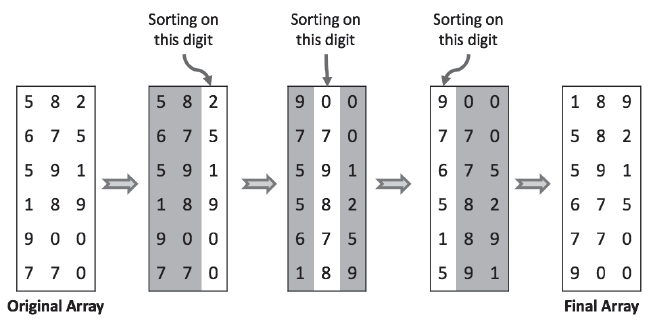
\includegraphics[width=1\textwidth]{radix1.png}
\caption{Exemplo execução do \textit{Radix Sort}. Fonte: \cite{ritambhara_radix_nodate}}
\label{fig:radix1}
\end{figure}

O \textit{Merge Sort} é um algoritmo de ordenação que se baseia na técnica "dividir para conquistar". Essa técnica consiste em dividir um problema em pedaços menores, continuar dividindo os menores recursivamente até chegar a um tamanho mínimo, resolvê-los e uni-los novamente.

No caso do algoritmo, podemos considerar o problema como sendo uma lista de inteiros a ser ordenada. Esta lista é dividida pela metade, criando duas sub-listas, que por sua vez também serão divididas até chegarmos a várias listas que contenham apenas um elemento. Em seguida, comparamos os elementos obtidos, ordenando-os e unindo-os aos poucos em novas sub-listas que mais tarde formarão uma nova lista ordenada.

Considerando que o \textit{Merge Sort} é um potencial algoritmo auxiliar do \textit{Radix Sort}, este trabalho visa explicar os passos que provam a estabilidade da interação entre esses dois algoritmos. Sendo assim, o algoritmo auxiliar deve ajudar o algoritmo principal a ordenar listas de elementos sem desfazer ordenações de partes já realizadas, não ordenando elementos de dígitos iguais em comparação e não inserindo elementos ou retirando elementos da lista inicial.

Mostraremos através da lógica de predicados, utilizando as regras do Cálculo de Sequentes com auxilio da ferramenta \textit{Prototype Verification System} para formalizar demonstrações implementadas.

\begin{figure}[!h]
\centering
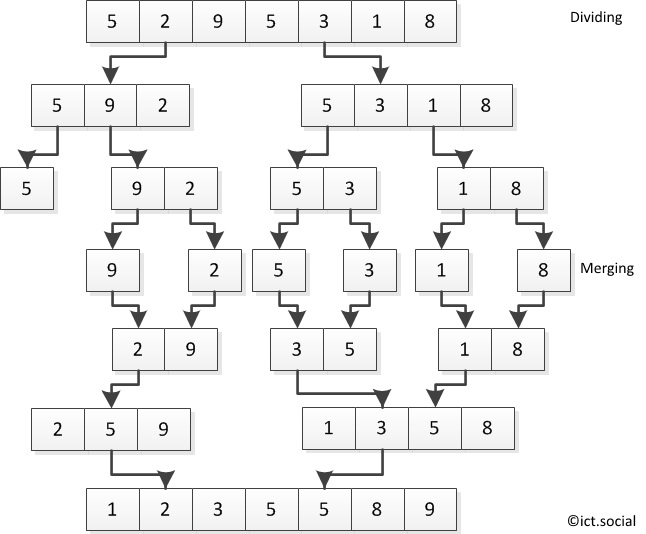
\includegraphics[width=0.8\textwidth]{merge1.jpg}
\caption{Exemplo execução do \textit{Merge Sort}. Fonte: \citep{capka_ict.social_nodate}}
\label{fig:mergex1}
\end{figure}

\section{Especificação do Problema e Explicação do Método de Solução}
\label{sec:Especificacao}

Com o objetivo de provar a estabilidade do algoritmo \textit{Merge Sort} em integração ao \textit{Radix Sort}, foram formalizadas três propriedades do algoritmo principal que possibilitam a utilização do auxiliar em complemento ao método de ordenação.

\subsection{Questão 1}
\label{sec:espec-q1}

A primeira questão consiste em demonstrar que para qualquer número natural \textbf{n}, n será sempre menor que dez elevado ao número de dígitos de n.

\begin{equation}
    \begin{split}
        \forall n \in \mathbb{N}, 10^{n\_digits(n)} > n
    \end{split}
    \label{eq:func}
\end{equation}

Para a solução deste problema utilizou-se indução matemática
forte sobre $n$.

\subsection{Questão 2}
\label{sec:espec-q2}

Na segunda questão quer-se mostrar que o \textit{merge} preserva os dados, ou seja, que o \textit{merge} apenas reordena ou permuta os elementos presentes nas duas listas fornecidas. Portanto, os mesmos elementos presentes no merge de duas listas quaisquer, sem adição nem remoção de elementos, também estão presentes no \textit{append} dessas duas listas.
\begin{alltt}
  merge_permutes : CONJECTURE
  FORALL(l1, l2 : list[nat], d : nat):
  permutations(append(l1,l2),merge(l1,l2,d))
\end{alltt}

A permutação, nesse caso, pode ser decomposta com a função de ocorrência de um determinado elemento $x$ na lista.
\begin{alltt}
  permutations(l1,l2:list[nat]):bool =
	FORALL (x:nat): occurrences(l1)(x) = occurrences(l2)(x)
\end{alltt}

Sendo o merge definido como
\begin{alltt}
merge(l1, l2 : list[nat], d : nat) : RECURSIVE list[nat] =
IF null?(l1) OR null?(l2) THEN append(l1, l2)
ELSIF d_nth(car(l1),d) <= d_nth(car(l2),d) 
    THEN cons(car(l1), merge(cdr(l1),l2, d))
ELSE cons(car(l2), merge(l1, cdr(l2), d))
ENDIF
MEASURE length(l1) + length(l2)
\end{alltt}

De modo que a função de ocorrências calcula o número de vezes que um elemento $x$ aparece em uma determinada lista.
\begin{alltt}
occurrences(l)(x): RECURSIVE nat =
IF  null?(l) THEN 0
    ELSIF 
      car(l) = x THEN 1 + occurrences(cdr(l))(x)
      ELSE
	occurrences(cdr(l))(x)
	ENDIF
MEASURE length(l)
\end{alltt}

A estratégia de solução deste problema foi a indução forte sobre
a soma dos tamanhos das listas $l1$ e $l2$.

\subsection{Questão 3}
\label{sec:espec-q3}
Na terceira e última questão é requisitada uma prova da estabilidade da função \textit{merge sort}. Assim, é necessário provas que, dada uma lista ordenada até o dígito $d$ (não inclusivo), quando é aplicada a função \textit{merge sort} no dígito d, essa lista é então ordenada até o dígito $d+1$ (não inclusivo). 
\begin{alltt}
  merge_sort_d_sorts : CONJECTURE
   FORALL(l : list[nat], d : nat) :
    is_sorted_ud?(l,d)  => 
    is_sorted_ud?(merge_sort(l,d),d+1)
\end{alltt}

Para essa prova, tem-se que a função \textit{is\_sorted\_ud?} retorna um valor verdadeiro quando qualquer elemento de índice $i$, tal que $i < j$, é menor que qualquer elemento de índice $j$, analisado até o dígito $d$. Por esse motivo, é verificado o resto da divisão do elemento por $10^d$.
\begin{alltt}
 is_sorted_ud?(l : list[nat], d : nat) : bool =
 FORALL(i : below[length(l)], j : below[length(l)] | i <= j) :
    rem(10^d)(nth(l,i)) <= rem(10^d)(nth(l,j))
\end{alltt}


A solução deste problema foi realizada por indução forte sobre o
tamanho da lista $l$.

\section{Explicação das Soluções e Formalização}
Em todos os casos o uso da estratégia de indução nos fornece uma
hipótese extra no conjunto de fórmulas no antecedente dos problemas
relacionada à hipótese da indução. Uma vez que a especificação da
estratégia de solução é o primeiro passo de cada prova, inicia-se
cada uma delas com a hipótese de indução disponível para ser
manipulada e com o consequente instanciado com um determinado
valor (arbitrário) que será o objeto da prova.

\label{sec:Solucoes}
\subsection{Questão 1}
\label{sec:sol-q1}

    Para a primeira prova, pode-se iniciar a resolução expandindo a definição da função \textit{n\_digits}.
    Nesse caso, como é uma função com resultados diferentes de acordo com uma condição de valor de $x1$,
    são criados dois ramos, um quando o valor de $x1$ é menor que $10$ e outro ramo quando $x1 >= 10$.
    
    Quando $x1 < 10$ temos o caso baso. Nessa situação de mais simples prova, temos que provar
    \begin{alltt}
    x!1 < 10 IMPLIES 10 ^ 1 > x!1
    \end{alltt}
    Por ser uma implicação, a condição vai para o antecedente, de forma que tem-se que $x1 < 10$, e assim é trivial perceber que $x1 < 10^1$
    
    Para o outro ramo, por \textit{n\_digits} ser uma função recursiva, é necessário provar que
    \begin{alltt}
    10 ^(1 + n_digits(ndiv(x!1, 10))) > x!1
    \end{alltt}
    Para isso, será necessário utilizar a hipótese da indução forte. Assim, no antecedente é obtido que 
    \begin{alltt}
    10 ^(n_digits(ndiv(x!1, 10))) > ndiv(x!1, 10)
    \end{alltt}
    Sabendo pelas definições que
    \begin{alltt}
    rem(10)(x!1) < 10
    x!1 = 10 * q + rem(10)(x!1)
    \end{alltt}
    E lembrando que estào sendo trabalhados números naturais, ao dividir o consequente por 10, temos o mesmo resultando que o antecedente, concluindo a prova do consequente. 

\subsection{Questão 2}
\label{sec:sol-q2}
    É necessário provar que, para quaisquer listas $x1$ e $x2$, escolhido um dígito $d$, temos que todo elemento presente em no \textit{append} de $x1$ e $x2$ também deve estar no \textit{merge} de $x1$ e $x2$ e vice-versa. Para isso, expandindo a definição da função \textit{merge}, é necessário provar 4 diferentes casos, visto que essa função é construída por uso de condicionais, portanto, para cada condição dever-se-á fechar a prova. 
    
    Nos dois primeiros casos, uma das listas é vazia, ou seja, $x1$ ou $x2$ não contém elementos. Por conseguinte, o \textit{merge} é definido como sendo um $append(x1, x2)$, dessa forma é fácil provar que $append(x1, x2)$ possuem exatamente os mesmos elementos que $append(x1, x2)$.
    
    No terceiro caso, obtido pela situação em que o primeiro elemento de $x1$ é menor que o primeiro elemento de $x2$ de acordo com o $d$-ésimo dígito, é necessário provar que 
    \begin{alltt}
        permutations(append(x!1, x!2),
                     cons(car(x!1), merge(cdr(x!1), x!2, d)))
    \end{alltt}
    Analisando a definição da função \textit{append}, nota-se que quando $x1$ não é vazia, a função é recursiva, de modo que se iguala a 
   \begin{alltt}
        permutations(cons(car(x!1), append(cdr(x!1), x!2)),
                     cons(car(x!1),  merge(cdr(x!1), x!2, d)))
    \end{alltt}
    Assim, já que está sendo utilizada a indução forte, tem-se no antecedente que para duas listas $y1$ e $y2$, $permutations(append(y1, y2), merge(y1, y2, d)))$,
    somente quando a soma dos seus tamanhos seja menor que a soma dos tamanhos de $x1$ e $x2$. Usando $y1$ igual a $cdr(x1)$, ou seja, a lista $x1$ sem o seu primeiro elemento e $y2$ igual a $x2$, a soma dos tamanhos de $cdr(x1)$ e $x2$ é menor que a soma dos tamanhos de $x1$ e $x2$. Utilizando a conclusão de que 
   \begin{alltt}
    permutations(append(cdr(x1), x2), merge(cdr(x1), x2, d)))
    \end{alltt}
    é verdadeira e utilizando o lema 
    \begin{alltt}
     cons_of_perm_is_permutation : LEMMA
        FORALL (l1, l2:list[nat], x:nat): 
               permutations(l1, l2) 
                  IMPLIES permutations(cons(x,l1), cons(x,l2))
    \end{alltt}
    sendo instanciado de forma que
    \begin{alltt}
permutations(append(cdr(x!1), x!2), merge(cdr(x!1), x!2, d)) 
    IMPLIES 
    permutations(cons(car(x!1), append(cdr(x!1), x!2)), 
        cons(car(x!1),  merge(cdr(x!1), x!2, d)))
    \end{alltt}
    temos assim a prova desse ramo.
    
    Para o último caso, obtido pela situação em que o primeiro elemento de $x2$ é menor que o primeiro elemento de $x1$ de acordo com o $d$-ésimo dígito, é necessário provar que 
    \begin{alltt}
    permutations(append(x!1, x!2),
        cons(car(x!2), merge(x!1, cdr(x!2), d)))
    \end{alltt}
    Aqui, devida a forma de definição da função \textit{append}, não é possível usar os mesmo passos utilizados para a prova do ramo anterior. Portanto, usa-se a expansão da definição da função \textit{permutations}, além de um novo lema
    \begin{alltt}
    occurrences_of_app : LEMMA
        FORALL (l1,l2:list[nat], x : nat) : 
            occurrences(append(l1, l2))(x) =
            occurrences(l1)(x) + occurrences(l2)(x)
    \end{alltt}
    Por essa lema é obtido que para quais quer listas $l1$ e $l2$, a soma da ocorrência de elementos $x$ em um \textit{append} dessas listas é igual a soma das ocorrências desses mesmo elementos em cada lista individualmente. Como no passo anterior, usando o antecedente dado pela indução forte, mas realizando a quebra na lista $x2$, temos que 
    \begin{alltt}
    permutations(append(x!1, cdr(x!2)), 
        merge(x1, cdr(x!2), d)))
    \end{alltt}
    Assim, obtém-se que 
    \begin{alltt}
    occurrences(x!1)(x) + occurrences(cdr(x!2))(x) = 
        occurrences(merge(x!1, cdr(x!2), d))
    |-------------
    occurrences(x!1)(x) + occurrences(x!2)(x) = 
        occurrences(cons(car(x!2), merge(x!1, cdr(x!2), d)))
    \end{alltt}
    Portanto, expandindo a \textit{occurrences} obtém-se a única diferença, $car(x!2)$, entre antecedente e consequente, mas que aparece nos dois lados da igualdade no consequente, concluindo a prova.

\subsection{Questão 3}
\label{sec:sol-q3}
    Como definida na Seção \ref{sec:espec-q3}, é requisitada a prova da estabilidade do \textit{merge sort}. Para isso, utilizando dedução forte novamente, expande-se a definição de \textit{merge sort}, assim são obtidos dois casos. No caso base, o tamanho da lista é menor ou igual a um, portanto ela está ordenada até o $d + 1$-ésimo dígito. Para o outro caso, é necessário concluir que
    \begin{alltt}
is_sorted_ud?(
    merge(
        merge_sort(prefix(x!1, floor(length(x!1) / 2)), d), 
        merge_sort(suffix(x!1, floor(length(x!1) / 2)), d), 
     1 + d)
    \end{alltt}
    Para isso, é preciso do lema que diz que o \textit{merge} preserva a ordenação
    \begin{alltt}
merge_preserves_sort : LEMMA
    FORALL(l1,l2 : list[nat], d : nat):
    (is_sorted_ud?(l1,d+1) AND is_sorted_ud?(l2,d+1) AND
        FORALL(i:below[length(l1)], j:below[length(l2)]) :
        rem(10^d)(nth(l1,i))  <= rem(10^d)(nth(l2,j)) )  =>
        is_sorted_ud?(merge(l1,l2,d),d+1)
    \end{alltt}
    Como esse lema é composto por uma implicação, a condição de implicação, então, vai para o consequente quando realizada a simplificação. Assim, são gerados três ramos que devem ser provados.
    
    Em dois deles, é necessário provar que o \textit{merger sort} do prefixo e do sufixo estão ordenados até o dígito $d + 1$. Utilizando, então, a hipótese da indução forte, por o prefixo e sufixo terem tamanho menor que a lista toda, temos a conclusão que o \textit{merge sort} do prefixo e do sufixo estão ordenados até o dígito $d + 1$. No entanto, pela hipótese de indução se tratar de uma implicação, fica necessário provar que o prefixo e o sufixo estão ordenados até o $d$-ésimo dígito. É possível, portanto, usar um dos antecedentes dado por uma simplificação da implicação que se quer provar.
   \begin{alltt}
    is_sorted_ud?(x!1, d)
    \end{alltt}
    Como a lista $x1$ está ordenada até o dígito $d$, temos que, usando os lemas dos conteúdos do sufixo e prefixo, o prefixo e sufixo também estão ordenados, completando a prova desses ramos. 
    
    Para o último ramo, é preciso provar que qualquer elemento do \textit{merge sort} pelo $d$-ésimo dígito do prefixo é menor que qualquer elemento do  \textit{merge sort} pelo $d$-ésimo dígito do sufixo . Sabendo que o \textit{merge sort} permuta, ou seja, conserva os elementos da lista original e conhecendo a relação de indexação dos elementos do prefixo e sufixo com a lista $x1$ original, sendo o corte no meio da lista qualquer elemento da metade para baixo (prefixo) terá índice menor que qualquer elemento da metade para cima (sufixo), é possível mostrar, usando o lema que as permutações de uma lista preservam seu conteúdo e fazendo as substituições necessárias, que, por a lista original $x1$ estar ordenada até o $d$-ésimo dígito, qualquer elemento do \textit{merge sort} no $d + 1$-ésimo dígito do prefixo de $x1$ será menor que qualquer elemento do \textit{merge sort} no $d + 1$-ésimo dígito do sufixo. 

\section{Conclusões}
\label{sec:Conclusao}

Neste trabalho foram demonstradas algumas propriedades relacionadas
à correção do \textit{Radix Sort} e de seu algoritmo auxiliar, o
\textit{Merge Sort}. Uma vez que o \textit{Radix Sort} executa a
ordenação por algarismos, iniciamos com uma prova relacionada com
a função \textit{n\_digits}, que nos fornece uma forma de isolar
uma certa quantidade de algarismos de um número natural, ignorando
o resto, o que a torna uma função cujo papel é essencial no algoritmo.

Em seguida realizamos uma prova relacionada com o algoritmo auxiliar
\textit{Merge Sort}, em particular com a parte \textit{"merge"}
do algoritmo, onde duas listas ordenadas são intercaladas. Aqui
demonstrou-se que o \textit{merge} não insere nem remove elementos
da lista, o que é uma característica esperada de um algoritmo
de ordenação, e que portanto deve se refletir no algoritmo auxiliar
utilizado.

Por fim, mostramos que o \textit{Merge Sort} é estável, ou seja,
ele não modifica a ordem de elementos iguais na lista. Esta
propriedade não é esperada e nem tampouco necessária a todos
os algoritmos de ordenação. Entretanto, ela é necessária ao algoritmo
auxiliar do \textit{Radix Sort}, visto que um "empate" entre dois
elementos até um dado algarismo não implica que ambos os elementos
sejam de fato iguais.

Com isto, foi possível completar a prova sobre a correção do
\textit{Radix Sort}, cujos outros enunciados já estavam previamente
finalizados no arquivo de provas, bem como experimentar um pouco
da prática relacionada a provas formais, que são uma ferramenta
essencial na garantia da qualidade de soluções algorítmicas para
problemas que, em muitos casos, podem se tratar de questões críticas e
com pouca tolerância a erros.

\bibliographystyle{pt-plainnat}	
\bibliography{radix}

\end{document}
